\documentclass[a4paper,11pt,twoside,openright]{Thesis}

\usepackage[japanese,master]{ThesisTemplate} 
%% オプション"japanese"を消すと英語化されます。
%% 論文種類は、phd, master, bachelor の3種類です。(デフォルトはphd)

\setcounter{secnumdepth}{3} % show subsubsection numbers

\putTitle{Title of your thesis}
\putAuthor{The Author}{Department of Physics, A University}
\date{\today}

\begin{document}
\maketitle
\frontmatter
\putAbstract{inputs/abst}
\tableofcontents

\mainmatter
\chapter{LHC ATLAS実験}
Large Hadron Collider(LHC)はスイス、ジュネーブにある欧州原子核研究機構(CERN)の地下100m,周長26.7kmのリングで構成される円形加速器である.最大で14TeVの重心系エネルギーで陽子陽子衝突させることが可能な,世界最大の陽子陽子衝突型加速器である.新粒子の探索や,ヒッグス粒子やトップクォーク等の質量が大きい粒子を多く生成できるので,結合定数などの精密測定も行うことが可能である.\\
LHCは2010年から運転を開始し,7TeVから8TeVの重心系エネルギーで2012年まで稼働した.この期間をLHC Run-1と呼び,瞬間最高ルミノシティは$0.77\times10^{34} \mathrm{cm^{-2}s^{-1}}$であった.その後,2013年から2015年までのシャットダウン期間で加速器のアップグレードを行い,2015年からは重心系エネルギー$13\mathrm{TeV}$でLHC Run-2が始まり,2018年まで続いた.Run-2の3年間で得られた積分ルミノシティは約$150\mathrm{fb}^{-1}$であった.\\
LHCは2年間のシャットダウン期間を経て2021年から重心系エネルギー$14\mathrm{TeV}$のLHC Run-3を予定している.Run-3が約3年間運転したのち,シャットダウン期間を挟んで,High Luminosity LHC(HL-LHC)が開始する予定である.

\section{ATLAS実験}
ATLAS実験はLHCの衝突点に設置されたATLAS検出器を用いて陽子陽子衝突から$\mathrm{TeV}$スケールまでの高エネルギー物理事象を探索する実験である.2012年には,LHC実験の1つであるCMS実験と共にヒッグス粒子を発見し,標準理論の完成お大きな役割を担った.世界最高エネルギーのLHCを使ったヒッグス粒子やトップクォークといった重い粒子の精密測定はATLAS実験の重要な目的の1つである.他にも超対称性粒子などの新粒子を発見することが特に大きな目的となっている.

\section{ATLAS検出器}
ATLAS検出器の全体図を示す.ATLAS検出器は高さ
This is the third page of the introductory chapter.

\chapter{Physics motivation}

\chapter{アップグレードに向けたモジュール量産}
前章で述べたように,HL-LHC計画に伴い,内部飛跡検出器のアップグレードが計画されている.本章では,それに伴う,モジュールの量産について\ref{sec:masspro}節で説明し,\ref{sec:pixmodule}節でモジュールの構成,要素であるシリコンセンサの原理を\ref{sec:sensor}節,フロントエンドASICについてを\ref{sec:rd53a}節で述べ,最後に\ref{sec:moduletest}節でモジュールの量産について必要な試験項目について説明する.\\

\section{モジュール量産とモジュールの構成}
\label{sec:masspro}
HL-LHC計画にあたって,内部飛跡検出器の総入れ替えを予定しているため,内部に用いるピクセルモジュールの量産が必要である.ここでは,Flex基板,フロントエンドASIC,シリコンピクセルセンサの3要素で構成された検出器をモジュールと呼ぶ.世界で約10000個のモジュールの量産が計画されており,日本グループはそのうちの約2000個を担当する予定になっている.\\
現在は,実機で用いるモジュールを量産するための準備として,プロトタイプ版のASICが4$\mathrm{Chip}$搭載されたモジュールで量産体制の確認が計画されている.プロトタイプ版の4$\mathrm{Chip}$モジュールは2020年2月ごろに完成が予定されている.\par
以下にピクセルモジュールの構造図を示す.モジュールはFlex基板,フロントエンドASIC,シリコンピクセルセンサの3要素で構成されている.図\ref{fig:module}にピクセル検出器の概念図を示す.センサとASICはバンプボンディングと呼ばれる手法で接合され,センサからのアナログ信号がASICによって処理される.また,ASICとFlex基板はワイヤボンディングと呼ばれる手法で接続されており,ASICで読み出された信号がFlex基板を通して伝達される仕組みになっている.\par

\begin{figure}[h]
  \centering
  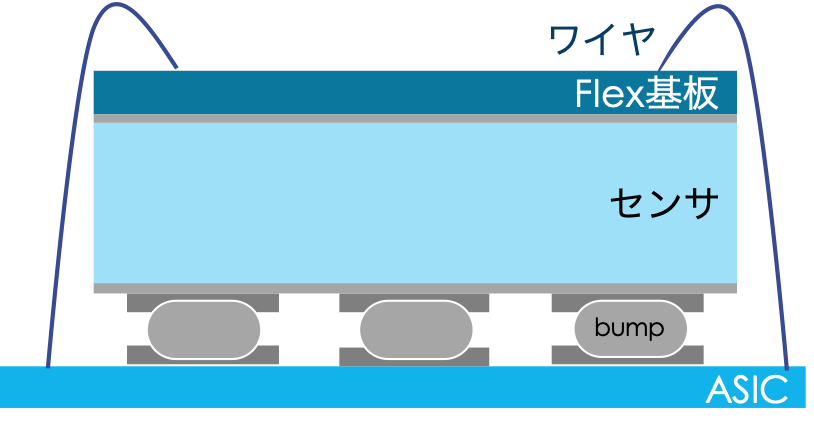
\includegraphics[width=8cm]{./figure/module.png}
  \caption{ピクセル検出器の概念図}
  \label{fig:module}
\end{figure}

\section{シリコンピクセルセンサ}
\label{sec:sensor}
この節では,ピクセル検出器を構成する要素の1つであるシリコンピクセルセンサについて説明する.

\subsection{シリコンピクセルセンサの原理}
シリコンセンサの動作原理は半導体に従う.この節では,半導体の基本原理と性質について述べる.\par
物質は導体,絶縁体,半導体の3種に分類することができる.これは,電気抵抗値によって決まっており,半導体は導体と絶縁体の中間の値をもつ.一般に室温で,$10^{-2}$から$10^9 \mathrm{\Omega cm}$の範囲に分類される.典型的な半導体物質にはシリコン,ゲルマニウム,ガリウムヒ素などがあげられる.

\subsubsection*{ドナーとアクセプタ}
半導体に不純物をドープすると,不純物準位が生じる.図\ref{fig:Donner}は$\ce{Si}$原子が5個の価電子を有する$\ce{As}$に痴漢された状況を模式的に示した図である.$\ce{As}$原子は隣接する4個の$\ce{Si}$原子と共有結合を形成し,残った電子は$\ce{As}$原子と弱く結合することで,適度な温度でイオン化されて伝導電子になる.この時の$\ce{As}$原子をドナーと呼ぶ.$\ce{Si}$は負電荷を持ったキャリアの負荷によりn型の半導体となる.同様に図\ref{fig:Acceptor}は3個の価電子をもつ$\ce{B}$が$\ce{Si}$に置換した場合を示す.4個の共有結合が$\ce{B}$の周囲にできるため,電子が1個取り込まれ,価電子帯に正に帯電した正孔が生じる.これがp型の半導体であり,$\ce{B}$はアクセプタと呼ばれる.

\begin{figure}[h]
  \centering
  \begin{minipage}[b]{0.45\linewidth}
    \centering
    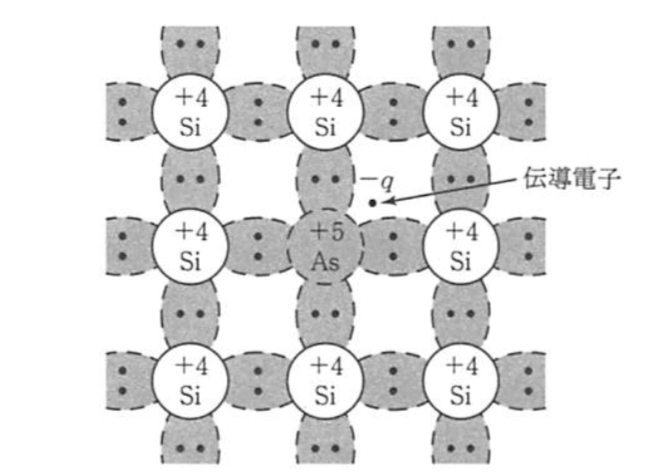
\includegraphics[width=8cm]{./figure/donner.png}
    \subcaption{ドナーをドープしたn型$\ce{Si}$}
    \label{fig:Donner}
  \end{minipage}
  \begin{minipage}[b]{0.45\linewidth}
    \centering
    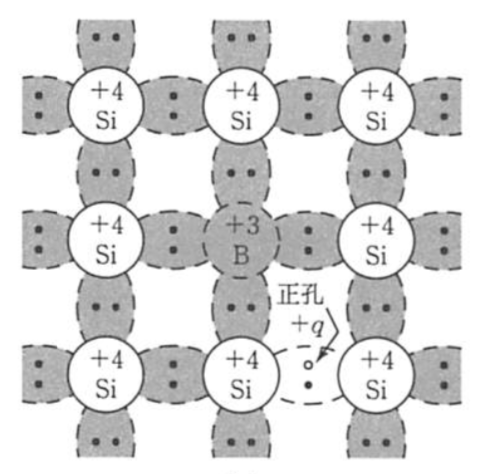
\includegraphics[width=5.8cm]{./figure/accepta.png}
    \subcaption{アクセプタをドープしたp型$\ce{Si}$}
    \label{fig:Acceptor}
  \end{minipage}
  \caption{ドープした半導体}
\end{figure}


\subsubsection*{pn接合と空乏化}
p型とn型の半導体が結合されると,接合部における大きなキャリア密度の勾配によってキャリアの拡散が起こる.p側からn側に向けて正孔が,n側からp側に向けて電子が拡散する.正孔がp側から拡散すると,結晶格子に固定されている負のアクセプタイオンが中和されずに接合近傍に残る.同様に,電子がn側から移動すると正のドナーイオンが接合近傍に残る.その結果,接合のp側には負の空間電荷が,n側には正の空間電荷が形成される.この空間電荷によって,電解が発生し,その向きは図\ref{fig:pn}のように正電荷側から負電荷側に向いている.\par

\begin{figure}[h]
  \centering
  \begin{minipage}[b]{0.45\linewidth}
    \centering
    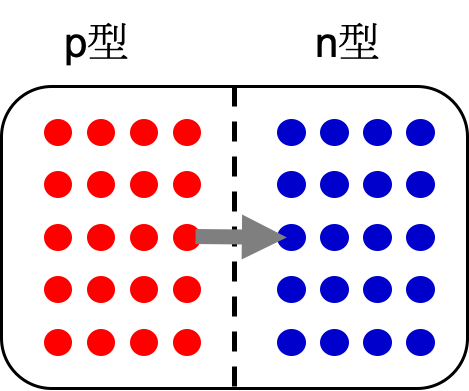
\includegraphics[width=4cm]{./figure/semiku1.png}
    \subcaption{過剰な電子と正孔が集まる}
  \end{minipage}
  \begin{minipage}[b]{0.45\linewidth}
    \centering
    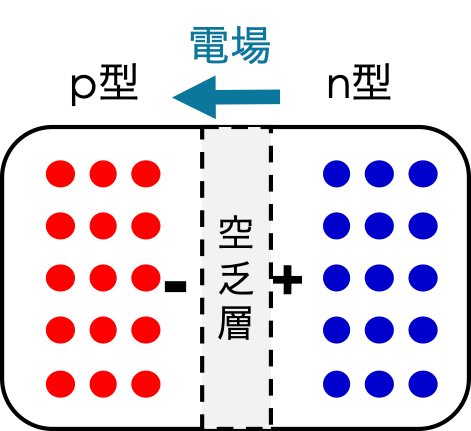
\includegraphics[width=4cm]{./figure/semiku2.png}
    \subcaption{空乏層が形成される}
  \end{minipage}
  \caption{pn接合半導体の空乏層概念図}
  \label{fig:pn}
\end{figure}


中世領域から接合部に近づくと,狭い遷移領域を経た上で,キャリアが存在しない領域が存在する.この領域を空乏層と呼ぶ.この空乏層の両端に生じる電位差は内臓電位$V_{bi}$と呼ばれ,アクセプタ濃度$N_A$,ドナー濃度$N_B$,不純物を含まない真性キャリア濃度$n_i$を用いて,式\ref{eq:bias}のように表される.\par
\begin{eqnarray}
  \label{eq:bias}
  V_{bi} = \frac{kT}{q} \ln \left( \frac{N_A N_D}{n_i^2} \right) 
\end{eqnarray}

空乏層幅は,静電ポテンシャルを示した一次ポアソン方程式\ref{eq:poisson}を解くことで,式\ref{eq:width}のような内部電位の関数にて表される.
\begin{eqnarray}
  \label{eq:poisson}
  \frac{d^2\Psi}{dx^2} \equiv -\frac{dE}{dx} = - \frac{q}{\epsilon_s}(N_D - N_A + p - n) \\
  \label{eq:width}
  W = \sqrt{ \frac{2\epsilon_s}{q} \left( \frac{N_A+N_D}{N_A N_D} \right) V_{bi}}
\end{eqnarray}

シリコンセンサはドープ量の少ない半導体にドープ量の多い半導体をインプラントしている($N_A \gg N_D$)ので,p側の空乏層幅はn側と比較して十分小さくなる.よって,式\ref{eq:width2}のように簡単に表すことができる.
\begin{eqnarray}
  \label{eq:width2}
  W \sim \sqrt{ \frac{2\epsilon_s V_{bi}}{q N_D} }
\end{eqnarray}

\subsubsection*{荷電粒子の検出}
荷電粒子が物質中の電子との衝突によって失うエネルギーは,Bethe-Blochの式\ref{eq:bb}で表される.\par
\begin{eqnarray}
  \label{eq:bb}
  - \frac{dE}{dx} = K z^2 \rho \frac{Z}{A} \frac{1}{\beta^2} \left[ \ln \left( \frac{2m_e c^2 \beta^2 \gamma^2 W}{I^2} \right) - \beta^2 - \frac{\delta(\gamma)}{2} \right]
\end{eqnarray}

入射した荷電粒子は物質中を通過する際に,物質の電子と相互作用することで,イオン化・励起し,電荷を生成する.この電荷をセンサが収集することで,通過した荷電粒子のエネルギーを知ることができる仕組みになっている.式\ref{eq:bb}より,$\beta \gamma \sim 3$付近で$-dE/dx$は最小となる.このような粒子をMinimum Ionization Particle(MIP)と呼ぶ.ここで,1MIPが150 $\mu m$厚のシリコンセンサを通過した場合を考える.MIPはシリコン中で多数の電子と相互作用し,その時に失うエネルギーの分布は式\ref{eq:landau}のようなランダウ分布になる.
\begin{eqnarray}
  \label{eq:landau}
  f(\lambda) = \frac{1}{\pi} \int ^{\infty} _0 \exp[-t (\ln t+\lambda) ] \sin(\pi t) dt
\end{eqnarray}

今回の場合の最頻値は,平均値の約0.7倍,シリコン中でのMIPのエネルギー損失の平均は,1.664 $\mathrm{MeV cm^2/g}$,シリコンの密度は2.329 $\mathrm{g/cm^3}$である.したがって,1MIPが損失するエネルギーは式\ref{eq:Emip}のように表せる.

\begin{eqnarray}
  E &=& 1.664 \times 3 \times 10^{-2} \times 2.329 \times 0.7 \nonumber \\
  \label{eq:Emip}
  &=& 8.14 \times 10^4 \mathrm{eV}
\end{eqnarray}

また,電子-正孔対生成に必要なエネルギーは3.62$\mathrm{eV}$であるから,生成され電子-正孔対の数は式\ref{eq:thr}のようになる.
\begin{equation}
  \label{eq:thr}
  E / 3.62 = 22500
\end{equation}


\subsection{バイアス構造}
シリコンピクセルセンサには,製造時に良品不良品を選別するための高電圧用のバイアス構造が備わっている.\par
バンプボンディングの前にセンサのみの試験を行い,動作不良センサを取り除く品質評価の工程がある.このピクセルセンサ評価方法として,IV測定がある.IV測定には全てのピクセルがGNDに落とされている必要があり,また,各ピクセルは分離されている必要がある.そのための構造がバイアスレールとPolySi抵抗である.ピクセル間にバイアスレールを起き,そこから各PolySi抵抗を引くことで,各ピクセルはGNDと同電位とすることができ,各ピクセルは抵抗によって分離される.\par

\subsection{今回使用したシリコンピクセルセンサ構造}
本論文で扱うピクセルセンサの表面構造について述べる.図\ref{fig:sensor}は,上から見たセンサの様子である.ピクセルセンサは2次元的に電極が配列されており,センサのみのテストのためにバイアスレールが敷かれている.本論文で用いたピクセルセンサは図\ref{fig:sensor}で示すように,row番号0-96はバイアスレールが存在せず,col番号96-192はバイアスレールが存在する構造になっている.

\begin{figure}[h]
  \centering
  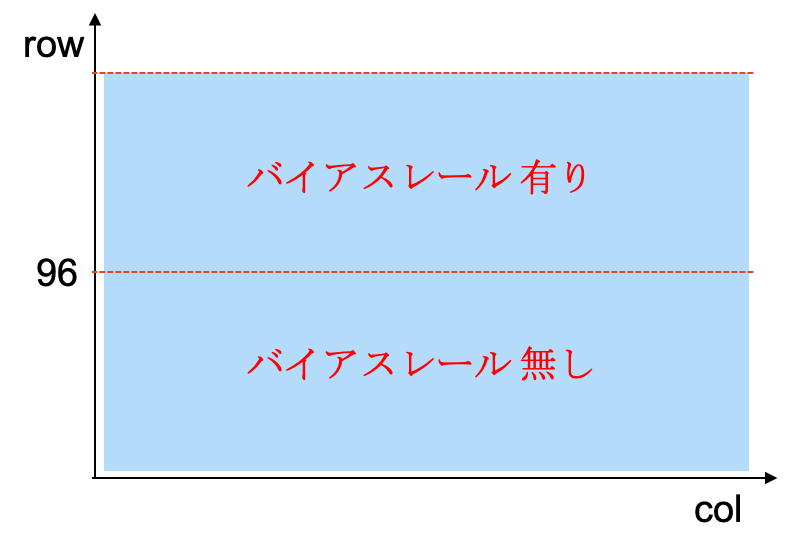
\includegraphics[width=7cm]{./figure/sensor.png}
  \caption{センサの構造.バイアスレールの有無}
  \label{fig:sensor}
\end{figure}


\section{HL-LHC ATLAS実験用新型ASIC・RD53A}
\label{sec:rd53a}
この節では,モジュールを構成する要素の1つであるASICについて述べる.ピクセル検出器からの信号は,検出器に直接接続された電気回路で最初に処理される.この電気回路をフロントエンドエレクトロニクスと呼ぶ.この回路は,全て専用の信号読み出し用ASIC内に実装されている.そのため,フロントエンドASICと呼ぶこともあるが,以降ではASICと呼ぶことにする.この回路を用いて検出器からの微弱な電気信号を受け取り,計測用のシステムに最適化した応答をするように信号をアンプ回路や波形整形回路などで調整する.さらに,コンピュータでの解析処理や,データの保存のためにアナログ信号をデジタル信号に変換する.\par
本論文で用いたASIC・RD53AはHL-LHC ATLAS実験用に開発されたプロトタイプ版の新型ASICであり,前章で述べたような,高い放射線耐性と,高い位置分解能を達成する.以下に現行のATLAS検出器で用いられているASIC・FEI4とFEI3,プロトタイプ版新型ASIC・RD53Aの比較を示す.

\begin{table}[h]
  \centering
  \caption{現行のASIC2種と新型プロトタイプ版ASICの比較}
  \begin{tabular} {|l|cc|c|} \hline
    ASIC名 & FEI3 & FEI4 & RD53A \\ \hline \hline
    ピクセルサイズ & 50 $\times$ 400 $\mathrm{\mu m^2}$ & 50 $\times$ 250 $\mathrm{\mu m^2}$ & 50 $\times$ 50 $\mathrm{\mu m^2}$ \\
    ピクセルのチャンネル数 & 18 $\times$ 160 & 80 $\times$ 336 & 50 $\times$ 50 $\mathrm{\mu m^2}$ \\ 
    チップサイズ & 7.6 $\times$ 10.8 $\mathrm{mm^2}$ & 20.2 $\times$ 19.0 $\mathrm{mm^2}$ & 20 $\times$ 11.8 $\mathrm{mm^2}$\\ \hline
  \end{tabular}
  \label{tab:ASIC}
\end{table}


\subsection{レジスタ}
ASICには,アナログ回路とデジタル回路の振る舞いを調節するために,回路の動作を制御する設定値を保持するレジスタが存在する.RD53Aのレジスタは2種類存在し,全てのピクセルに共通の設定を保存するグローバルレジスタ(GR)と各ピクセルの設定値を保持するピクセルレジスタ(PR)がある.
\begin{itemize}
\item グローバルレジスタ\\
  RD53Aには137個のGRがあり,ピクセルに共通が閾値(threshold),回路のオンオフなどを設定することができる.
\item ピクセルレジスタ\\
  Synchronous Frontendには3 $\mathrm{bit}$,その他の2つのフロントエンドには8 $\mathrm{bit}$のレジスタがある.ピクセルのデジタル回路のオンオフや閾値(threshold)を設定することができる.
\end{itemize}


\subsection{RD53Aフロントエンドデザイン}
RD53Aはプロトタイプ版のため,Synchronous Frontend, Linear Frontend, Differential Frontendと,3つの異なるフロントエンドデザインが存在する.

\begin{figure}[h]
\centering
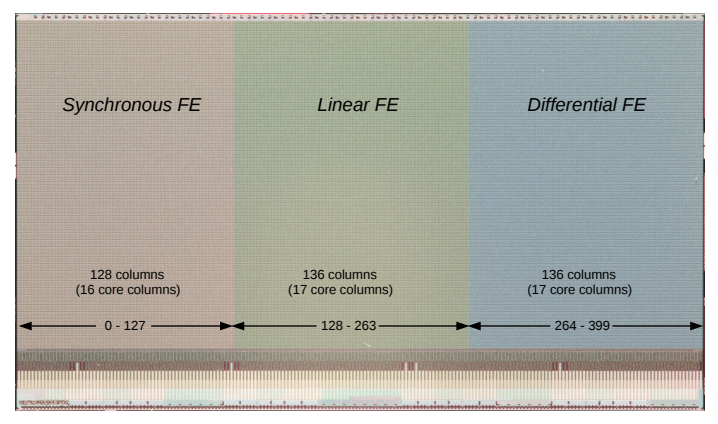
\includegraphics[width=8cm]{./figure/RD53A_FE.png}
\caption{RD53Aのフロントエンドデザイン}
\label{fig:RD53AFE}
\end{figure}

今回は実機で利用されることが予定されているDifferential Frontend(以下:Diff FE)のみを用いて研究を行なったため,それについて詳しく説明する.

\subsubsection*{Diff FEの仕組み}
3つのフロントエンドで大きく異なるのは,アナログ回路部分の構造である.Diff FEのアナログ回路構造を以下に示す.\par

\begin{figure}[h]
\centering
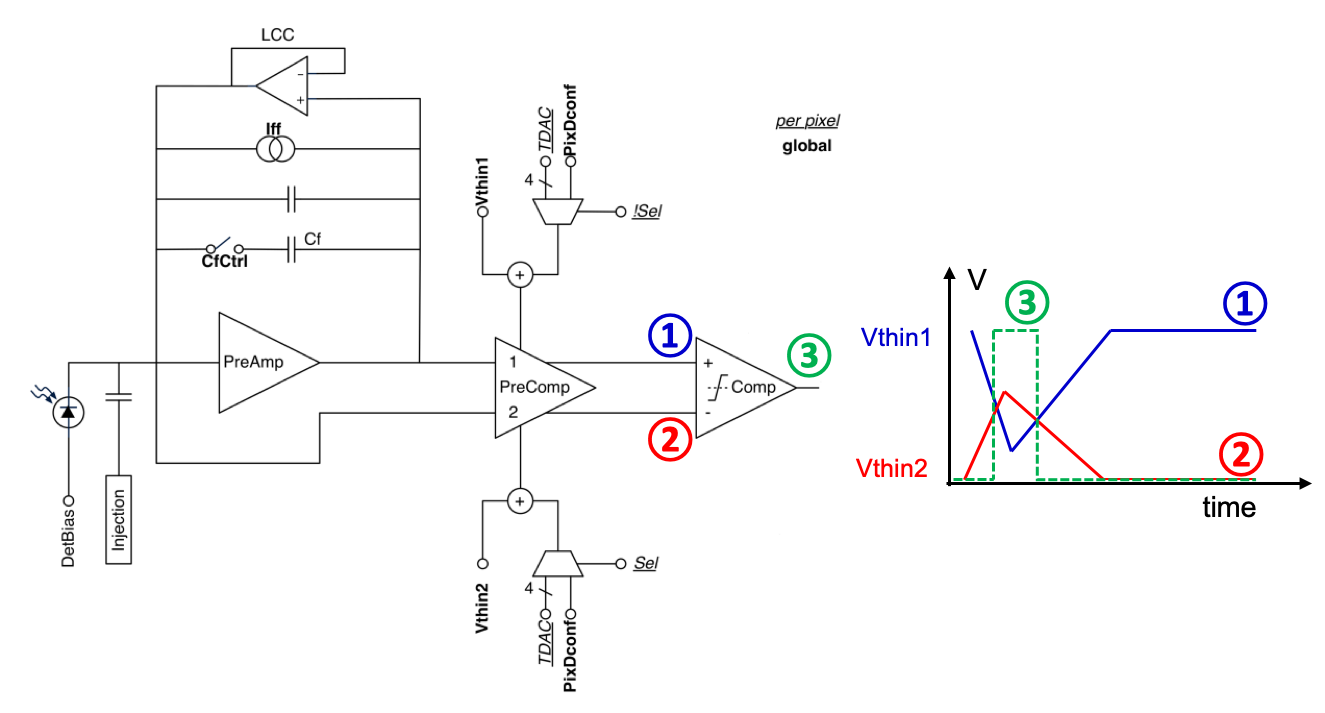
\includegraphics[width=12cm]{./figure/RD53A_DiffFE.png}
\caption{Diff FEのアナログ回路構造}
\label{fig:DiffFE}
\end{figure}

図\ref{fig:DiffFE}に示したように,Diff FEでは,RD53AのGR値である''DiffVthin1''と''DiffVthin2''で閾値を設定可能である.これらのGR値は,入力された信号(図\ref{fig:DiffFE}の赤い信号)と,それに対して反転増幅を行なった後の信号(図\ref{fig:DiffFE}の青い信号)それぞれに作用するオフセット電圧である.Diff FEはこれらの信号の差動によって,出力信号を定義しているため,オフセットを変化させることで,閾値を調整することができる.また,GR値である''DiffLccEn''で図中のCfCtrlのスイッチのオンオフを,''DiffLcc''でLCC回路に印加する電圧を設定することができる.

\subsection{RD53Aのデータ収集の仕組み}

\begin{figure}[h]
  \centering
  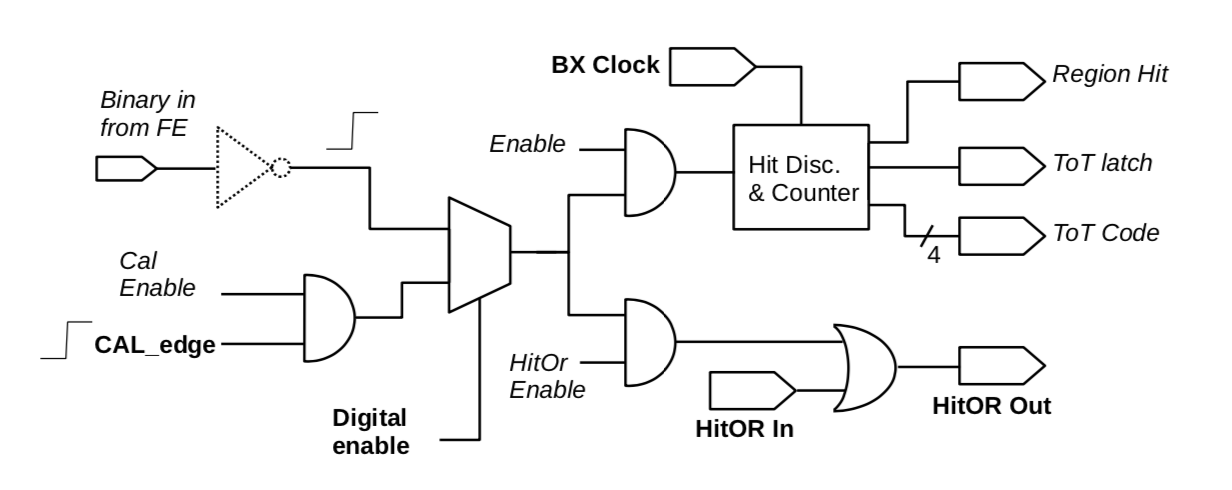
\includegraphics[width=13cm]{./figure/RD53Aproc.png}
  \caption{RD53Aのデータ収集の仕組み.全ピクセルに共通する信号が太字,ピクセルごとに記録されている信号が斜体文字になっている.}
  \label{fig:RD53Aproc}
\end{figure}

図\ref{fig:RD53Aproc}にRD53Aのデータ収集の仕組みを示す.まず,Hitとされる信号(センサからの信号)はBinary in from FEから,擬似パルスによる信号はCALedgeから入射する.各ピクセルごとに設定されている''Enable''がオンの場合,そのピクセルのデータは図中のHit Disc. \& Counterに入る.ここでは,Hitを検出したピクセルの位置(Region Hit)と,40$\mathrm{MHz}$のBX Clockに合わせて数え上げられるToT値とLatency値が記録されていく.

\subsubsection*{Time over Threshold(ToT)}
ToTとは,図\ref{fig:tot}で示すように,信号(Signal)が閾値(Threshold)を超えている間の時間を指す.

\subsubsection*{Latency}
Latencyとは,図\ref{fig:tot}で示すように,トリガが入力されてからどれだけ時間を遡ってデータ読み出しを行うかを指定する値をさす.

\begin{figure}[h]
  \centering
  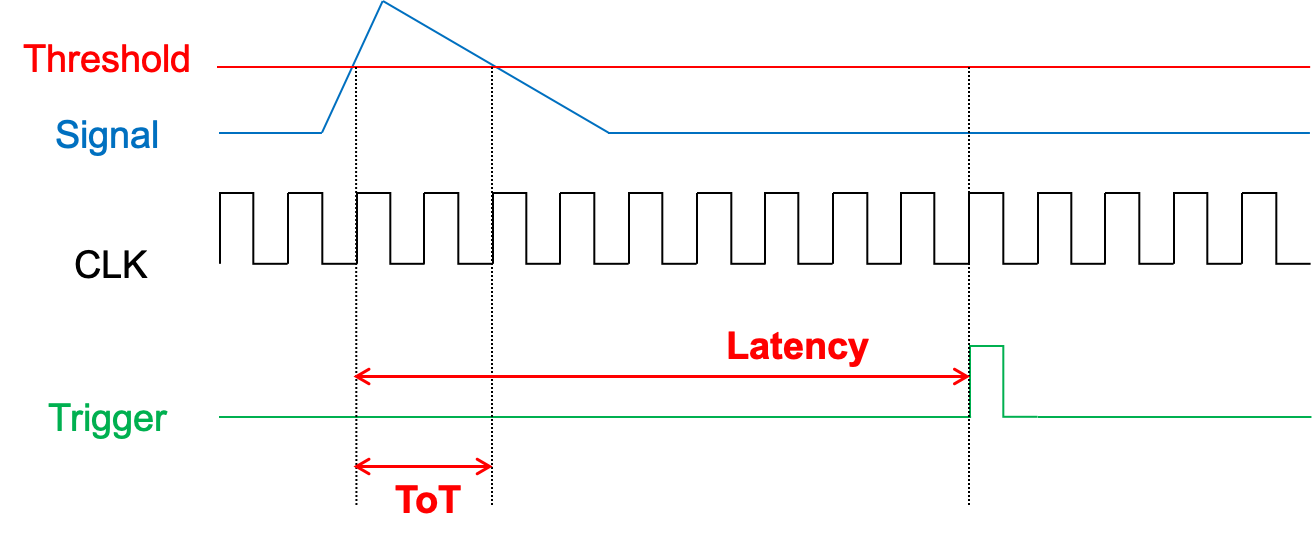
\includegraphics[width=13cm]{./figure/tot.png}
  \caption{信号が入力された時のToTとLatency}
  \label{fig:tot}
\end{figure}



\subsection{HitOR信号}
RD53Aには,現行のFEI4に実装されているセルフトリガ機能がない代わりに,HitORというセンサに荷電粒子が入射したタイミングで,出力される信号が存在する.HitOR信号出力する仕組みについて説明する.図\ref{fig:RD53Aproc}において,各ピクセルで設定されているレジスタ''HitOr Enable''がオンの場合,Hit信号または擬似パルス信号が入射すると,Hit Disc. \& Counterに入るのと同時に図中右下のHitOR Outから信号が出力される.これがHitOR信号である.\par

\begin{figure}[h]
  \centering
  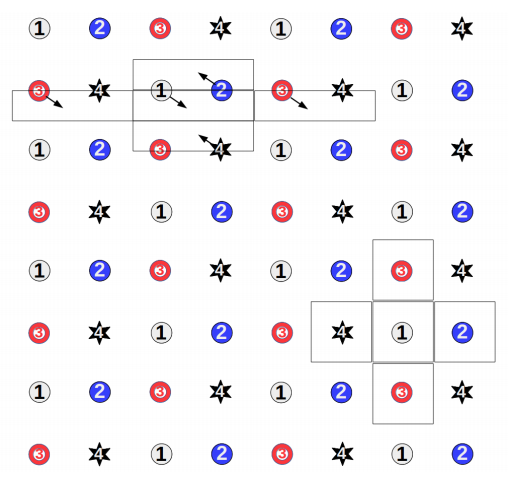
\includegraphics[width=8cm]{./figure/HitOR.png}
  \caption{HitOR信号のネットワーク図}
  \label{fig:HitOR}
\end{figure}

HitOR信号は4つのネットワークによって出力される.図\ref{fig:HitOR}はRD53Aの一部である$8 \times 8 \mathrm{pixel}$を示している.HitOR信号は,図\ref{HitOR}の各ピクセルに割り当てられている番号1-4ごとにまとめて読み出される.これを番号ごとにネットワークと呼ぶ.このネットワークは任意のネットワークに含まれるピクセルの上下に1つのネットワーク,左右に異なる2つのネットワークが存在するように配置されている.例えば,1番のネットワークのあるピクセルには,3番のネットワークが上下に存在し,左右には2番と4番のネットワークが存在するようになっている.このように配置されたネットワークごとに,HitORは読み出される仕組みになっている.

\section{モジュール量産に向けた品質性能試験}
\label{sec:moduletest}
量産されたモジュールは品質性能基準を達成するために,試験にかけられる.その試験項目の1つとして,本論文に関わる,粒子線に対する応答評価試験が存在する.

\subsection{粒子線に対する応答評価試験の意義}
HL-LHC ATLAS実験に向けたピクセル検出器量産に際して,全ての検出器モジュールに対して,品質管理のための試験を行う.この試験項目の1つとして,粒子線に対する応答評価試験が設けられている.前章でも述べたように,ピクセル検出器の各チャンネルとASICはバンプボンディングという手法で接続されている.このバンプボンディングに異常がないかどうかを確認するための試験が,ソーススキャンである.\par

\subsection{応答評価試験の手法}
応答評価試験には,主に2種類の手法がある.1つは,センサに荷電粒子が入射した時の信号を取得したタイミングでデータ取得を行う,セルフトリガと呼ばれる手法.もう1つは,センサの上にシンチレータ,その上に粒子線源を設置し,シンチレータに粒子線が入射した時の信号を取得したタイミングでデータ取得を行う手法である.今回はこれら2種類の手法を用いて応答評価試験を行い,どのような試験結果の振る舞いがなされるかの検証を行なった.\par
YARRソフトウェアには,外部トリガスキャンという機能が実装されているため,今回はこの外部トリガにHitOR信号を用いた手法をセルフトリガ,シンチレータに粒子線が入射した時の信号を用いた手法を外部トリガと呼ぶ.

\subsection{本研究の目的}
本研究では,シリコンピクセルセンサが接続されたHL-LHC ATLAS実験用新型ASIC搭載モジュールを用いて,2種類の手法で行なったの粒子線に対する応答評価試験結果について報告する.

\chapter{Object definition}

\chapter{Signal Optimisation}

\chapter{Background Estimation}

\chapter{Systematics}

\chapter{Results}

\chapter{Conclusion}


\chapter*{謝辞}

本研究を進める上でお世話になった方々にお礼申し上げます.指導教員である河野能知准教授には,研究の機会と環境を与えていただきました.また,素粒子実験に関わる知識だけでなくファームウェア,ソフトウェア,回路設計などのノウハウや,研究発表にあたって見やすく伝わりやすい資料作りについてご指導いただきました.毎週の研究室のミーティングでは,研究方針および手法について的確な指摘をいただき,研究をすすめることができました.心から感謝申し上げます.また,副指導教員で本論文の副査を務めていただきました高橋遼助教授にも感謝申し上げます.\par
ATLAS日本QA/QCグループの皆様に感謝いたします.大阪大学の廣瀬穣さんには,ミーティングの場だけでなく,ミーティング外でも時間をとって,ファームウェアの知識のない私に丁寧にご指導いただきましたことに感謝申し上げます.また,東京工業大学の生出秀行さんにも,ソフトウェアの開発やソースホルダの作成の際にたくさんのアドバイスをいただきました.感謝いたします.また,東工大の窪田ありささん,阪大の山家谷昌平さんには,同期として研究姿勢について多くを学ばせていただきました.東工大の松崎貴由さん.池亀遥南さんには,クーリングボックスにソースホルダを組み込むにあたって設計についての相談にのっていただきました.東工大の奥山広貴さんにはデータベースの使い方を丁寧に教えていただき,また阪大のLakmin Wickremasingheさんには回路設計についてアドバイスをいただきました.\par
お茶の水女子大学河野研究室の皆様に感謝申し上げます.藤本みのりさんには,データ取得を手伝っていただいたこと,ファームウェアとソフトウェアについての多くの知識を教えていただきました.浅井香奈江さんには,コーディング技術や,プロットの見せ方について多くの助言をいただきました.河野研究室卒業生の里吉陽奈子さんには,見やすい発表資料の作り方について大変参考にさせていただきました.また修士1年で同じATLAS日本QA/QCグループだった,釣希夢さん,前田実津季さんには発表資料や実験方針,ソフトウェアの設計など,多くの相談にのっていただき,大変感謝しています.\par
ATLASグループでは,KEKの中村浩二さん,筑波大学の原田大豪さんには,センサについての知識を教えていただいた上に,データ取得するにあたって多くの時間をとって協力してくださり大変感謝しています.また,東工大の金恩寵さん,潮田理沙さん,卒業生の中村優斗さんには学会などで会うたびによくしてくだいました.ありがとうございました.\par
最後に,何不自由ない学生生活,研究生活を実現してくたださった両親に深く感謝いたします.




\bibliography{./bib/IOPEXPORT_BIB}
\bibliographystyle{junsrt}
%\bibliography{./bib/HLLHC_BIB}
%\bibliography{./bib/ITK_BIB}

\appendix

\listoffigures
\listoftables

\end{document}

